\documentclass{article}
\usepackage{graphicx}

\title{Ketrampilan Pemrograman Chapter 2}
\author{nurulkamila1899 }
\date{October 2019}

\begin{document}

\maketitle

\section{Buatlah luaran huruf yang dirangkai dari tanda bintang, pagar atau plus dari
NPM kita. Tanda bintang untuk NPM mod 3=0, tanda pagar untuk NPM mod
3 =1, tanda plus untuk NPM mod3=2}
\begin{center}
    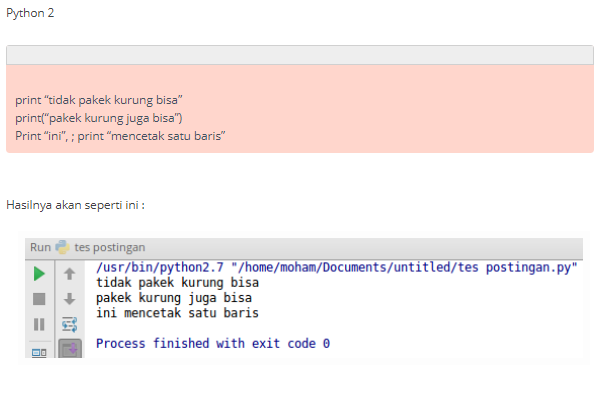
\includegraphics[width=.8\textwidth]{1.PNG}
\end{center}

\section{Buatlah program hello word dengan input NPM yang disimpan dalam sebuah
variabel string bernama NPM dan output sebanyak dua dijit belakang NPM,
contoh NPM : 113040087 maka akan ada output sebanyak 87 dengan tulisan ‘Hallo, 113040087 apa kabar?’} \\

NPM=int(input("masukkan NPM :")) \\
i=NPM%100 \\
for i in range(i): \\
    print("hello",NPM,"apa kabar?")\\
\begin{center}
    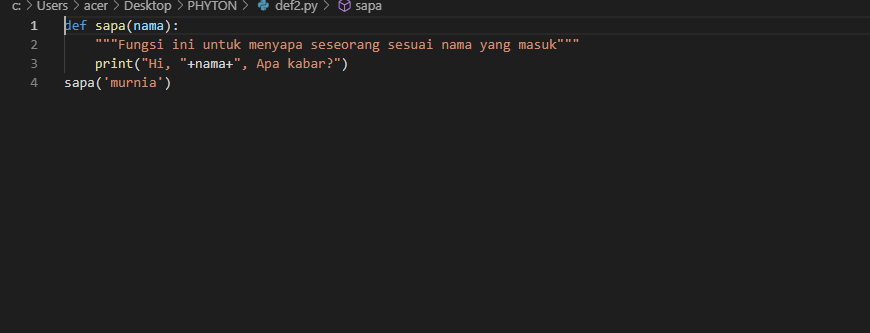
\includegraphics[width=.8\textwidth]{2.PNG}
\end{center}

\section{Buatlah program hello word dengan input nama yang disimpan dalam sebuah variabel string bernama NPM dan beri luaran output berupa tiga karakter belakang dari NPM sebanyak penjumlahan tiga dijit tersebut,} \\
NPM=input("Masukan Npm anda: ")\\
X =int (NPM[4])\\
Y =int (NPM[5])\\
Z =int (NPM[6])\\
hitung1 = X + Y + Z\\
hitung2 = X + Y + Z\\
while hitung1 > 0:\\
        print("Hallo, " , NPM[4:7], "Apa kabar ?")\\
        hitung1 = hitung1 -1 \\
print("...",str(hitung2),"kali(",str(X),"+",str(Y),"+"+str(Z),")...")\\
\begin{center}
    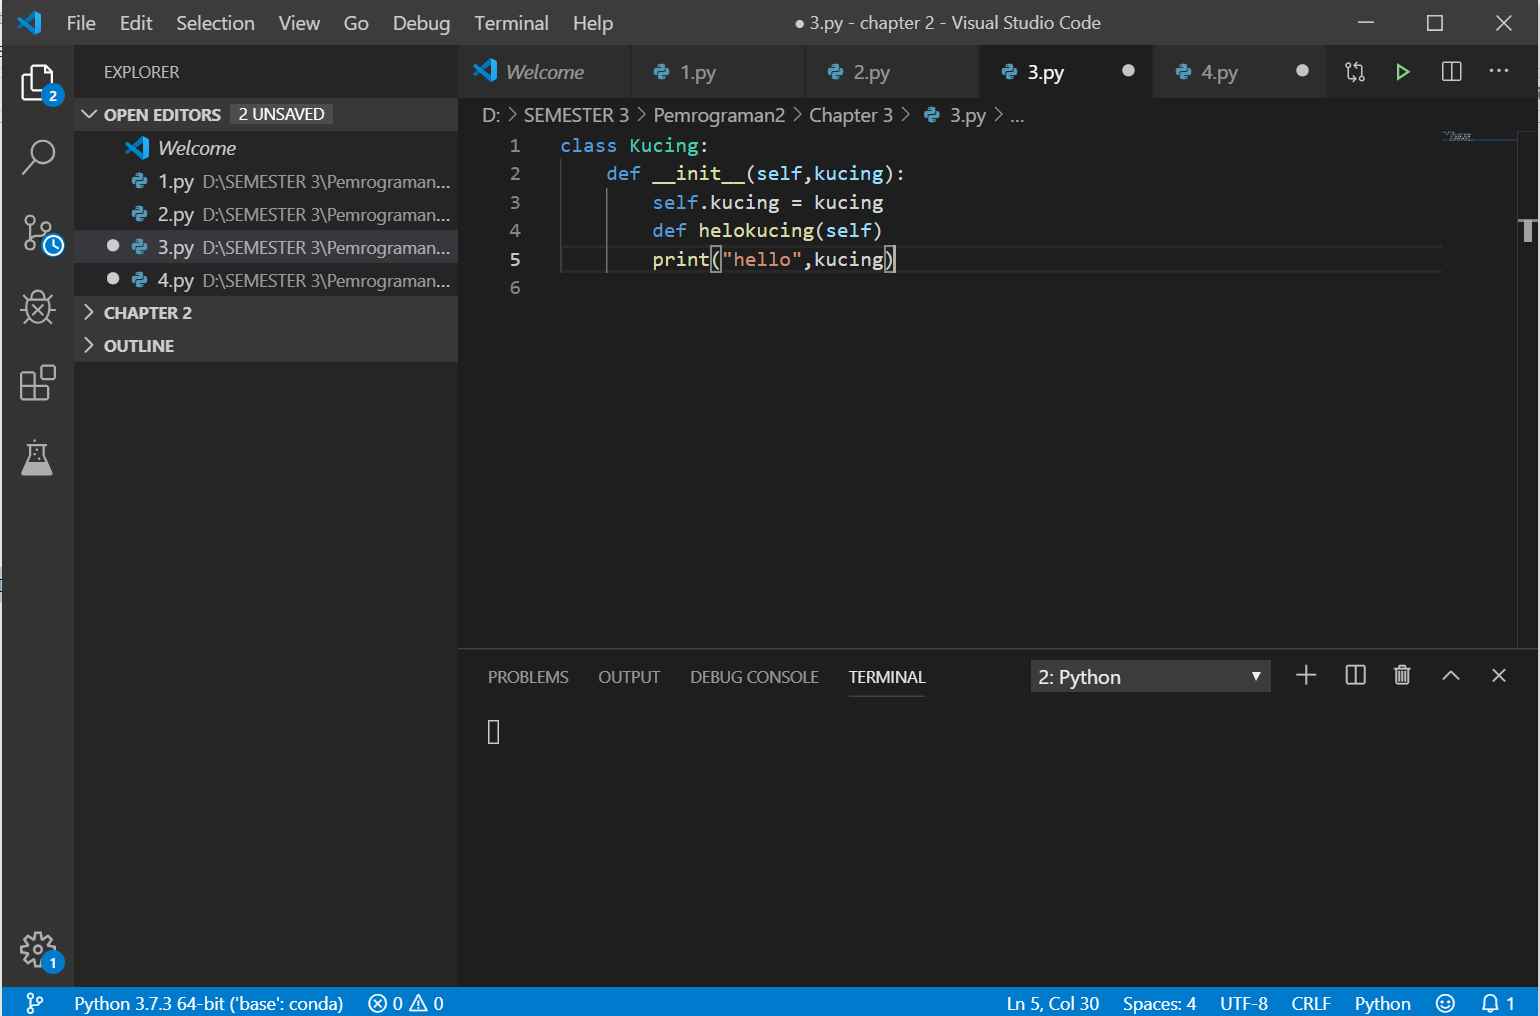
\includegraphics[width=.8\textwidth]{3.PNG}
\end{center}

\section{Buatlah program hello word dengan input nama yang disimpan dalam sebuah variabel string bernama NPM dan beri luaran output berupa digit ketiga dari belakang dari variabel NPM,}\\
NPM = input("Npm anda: ")\\
print("Hallo, ",NPM[4],"Apa kabar ?")\\
\begin{center}
    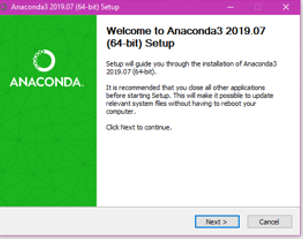
\includegraphics[width=.8\textwidth]{4.PNG}
\end{center}

\section{(untuk soal no 5 dan selanjutnya wajib menggunakan perulangan dan kondisi) buat program dengan mengisi variabel alfabet dengan nomor npm satu persatu berurut.} \\
i=0 \\
NPM = input("Npm anda: ")\\
while i <1:\\
    if len(NPM) <7:\\
        print("NPM anda kurang dari 7!")\\
        NPM = input("NPM anda: ")\\
    elif len(NPM) >7:\\
        print ("NPM lebih dari 7!")\\
        NPM = input ("NPM anda: ")\\
    else:\\
        i=1\\

A=NPM[0]\\
B=NPM[1]\\
C=NPM[2]\\
D=NPM[3]\\
E=NPM[4]\\
F=NPM[5]\\
G=NPM[6]\\

for this in A,B,C,D,E,F,G:\\
    print (this,end =" "),\\
\begin{center}
    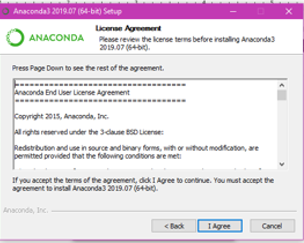
\includegraphics[width=.8\textwidth]{5.PNG}
\end{center}

\section{Dari soal no 5, Lakukan penjumlahan dari seluruh variabel tersebut,}\\
i=0\\
NPM = input("Npm anda: ")\\
while i <1:\\
    if len(NPM) <7:\\
        print("NPM anda kurang dari 7!")\\
        NPM = input("NPM anda: ")\\
    elif len(NPM) >7:\\
        print ("NPM lebih dari 7!")\\
        NPM = input ("NPM anda: ")\\
    else:\\
        i=1\\

A=NPM[0]\\
B=NPM[1]\\
C=NPM[2]\\
D=NPM[3]\\
E=NPM[4]\\
F=NPM[5]\\
G=NPM[6]\\

X=0\\

for this in A,B,C,D,E,F,G:\\
    X+=int(this)\\
print(X)\\
\begin{center}
    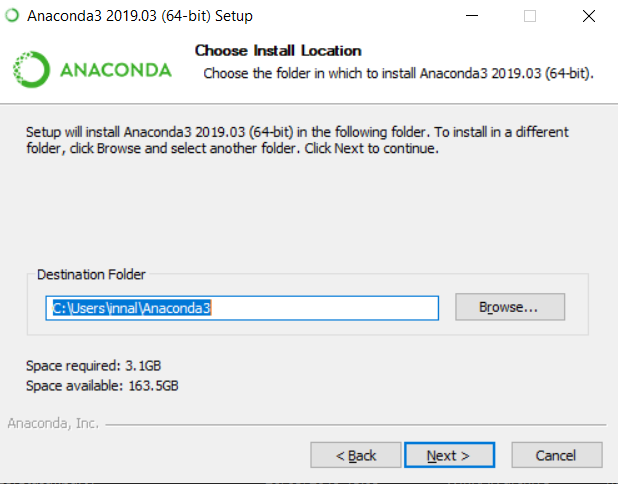
\includegraphics[width=.8\textwidth]{6.PNG}
\end{center}

\section{Dari soal no 5, Lakukan perkalian dari seluruh variabel tersebut,}\\
i=0\\
NPM = input("Npm anda: ")\\
while i <1:\\
    if len(NPM) <7:\\
        print("NPM anda kurang dari 7!")\\
        NPM = input("NPM anda: ")\\
    elif len(NPM) >7:\\
        print ("NPM lebih dari 7!")\\
        NPM = input ("NPM anda: ")\\
    else:\\
        i=1\\

A=NPM[0]\\
B=NPM[1]\\
C=NPM[2]\\
D=NPM[3]\\
E=NPM[4]\\
F=NPM[5]\\
G=NPM[6]\\

X=0\\

for this in A,B,C,D,E,F,G:\\
    X*=int(this)\\
print(X)\\
\begin{center}
    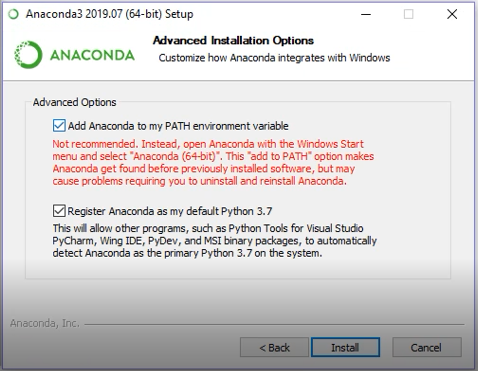
\includegraphics[width=.8\textwidth]{7.PNG}
\end{center}

\section{Dari soal no 5, Lakukan print secara vertikal dari NPM anda menggunakan variabel diatas}\\
i=0\\
NPM = input("Npm anda: ")\\
while i <1:\\
    if len(NPM) <7:\\
        print("NPM anda kurang dari 7!")\\
        NPM = input("NPM anda: ")\\
    elif len(NPM) >7:\\
        print ("NPM lebih dari 7!")\\
        NPM = input ("NPM anda: ")\\
    else:\\
        i=1\\

A=NPM[0]\\
B=NPM[1]\\
C=NPM[2]\\
D=NPM[3]\\
E=NPM[4]\\
F=NPM[5]\\
G=NPM[6]\\

X=0\\

for this in A,B,C,D,E,F,G:\\
    print(this)\\
\begin{center}
    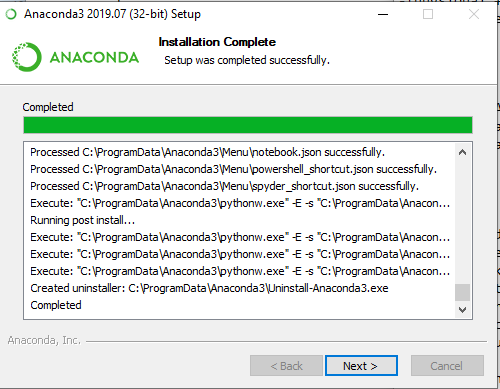
\includegraphics[width=.8\textwidth]{8.PNG}
\end{center}

\section{Dari soal no 5, Lakukan print NPM anda tapi hanya dijit genap saja.}\\
i=0\\
NPM = input("Npm anda: ")\\
while i <1:\\
    if len(NPM) <7:\\
        print("NPM anda kurang dari 7!")\\
        NPM = input("NPM anda: ")\\
    elif len(NPM) >7:\\
        print ("NPM lebih dari 7!")\\
        NPM = input ("NPM anda: ")\\
    else:\\
        i=1\\

A=NPM[0]\\
B=NPM[1]\\
C=NPM[2]\\
D=NPM[3]\\
E=NPM[4]\\
F=NPM[5]\\
G=NPM[6]\\

X=1\\

for this in A,B,C,D,E,F,G:\\
    
    if int (this)%2==0:\\
        if int(this)==0:\\
            this==""\\
        print(this,end=" ")\\
\begin{center}
    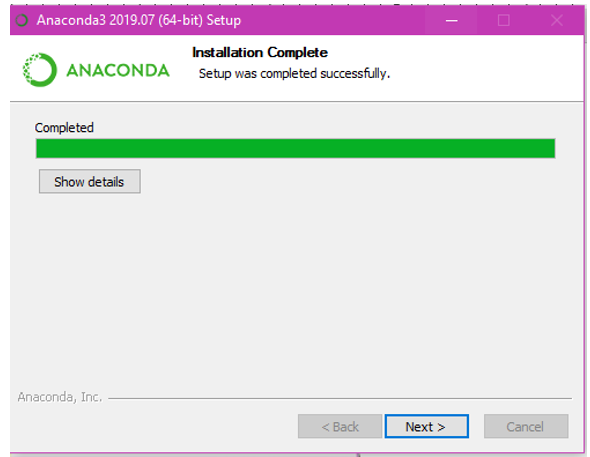
\includegraphics[width=.8\textwidth]{9.PNG}
\end{center}

\section{Dari soal no 5, Lakukan print NPM anda tapi hanya dijit ganjil saja.}\\
i=0\\
NPM = input("Npm anda: ")\\
while i <1:\\
    if len(NPM) <7:\\
        print("NPM anda kurang dari 7!")\\
        NPM = input("NPM anda: ")\\
    elif len(NPM) >7:\\
        print ("NPM lebih dari 7!")\\
        NPM = input ("NPM anda: ")\\
    else:\\
        i=1\\

A=NPM[0]\\
B=NPM[1]\\
C=NPM[2]\\
D=NPM[3]\\
E=NPM[4]\\
F=NPM[5]\\
G=NPM[6]\\

X=1\\

for this in A,B,C,D,E,F,G:\\
    
    if int (this)%2==0:\\
        if int(this)==0:\\
            this==""\\
        print(this,end=" ")\\
\begin{center}
    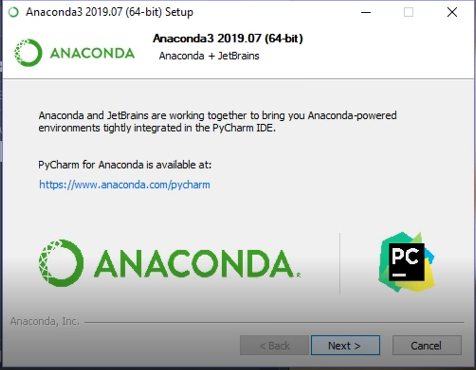
\includegraphics[width=.8\textwidth]{10.PNG}
\end{center}

\section{Dari soal no 5, Lakukan print NPM anda tapi hanya dijit yang termasuk bilangan prima saja.}\\
i=0\\
NPM = input("Npm anda: ")\\
while i <1:\\
    if len(NPM) <7:\\
        print("NPM anda kurang dari 7!")\\
        NPM = input("NPM anda: ")\\
    elif len(NPM) >7:\\
        print ("NPM lebih dari 7!")\\
        NPM = input ("NPM anda: ")\\
    else:\\
        i=1\\

A=NPM[0]\\
B=NPM[1]\\
C=NPM[2]\\
D=NPM[3]\\
E=NPM[4]\\
F=NPM[5]\\
G=NPM[6]\\

X=1\\

for this in A,B,C,D,E,F,G:\\
    
    if int (X)>1:\\
        for i in range(2,int(X)):\\
            if (int(X)% i)==0:\\
                break\\
        else:\\
            print (int(X),end =""),\\
\begin{center}
    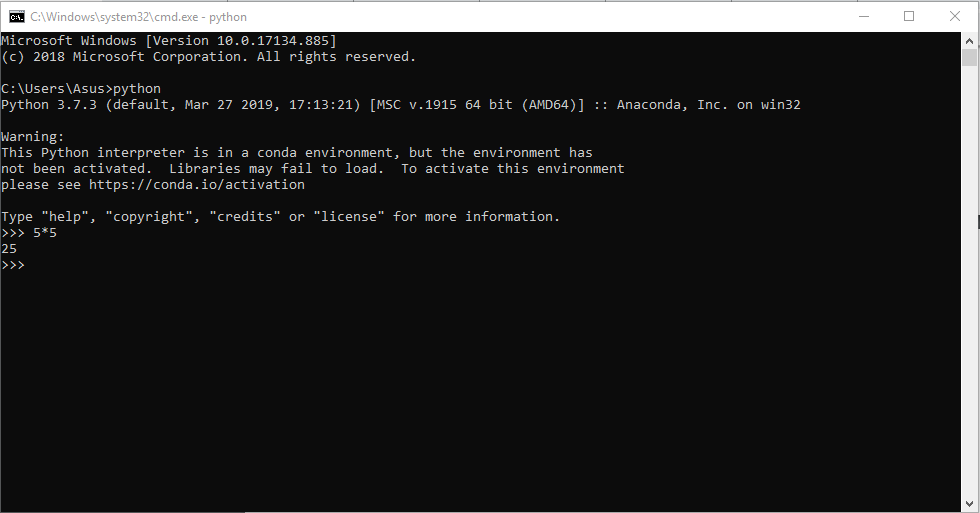
\includegraphics[width=.8\textwidth]{11.PNG}
\end{center}



\end{document}
